\documentclass[a4paper, 11pt]{book}
%\documentclass[a4paper, 11pt, draft]{book}

% Packages used
\usepackage{graphicx}
\usepackage{booktabs} % Good looking tables
\usepackage{url}
\usepackage{amsmath}
\usepackage[sorting=none]{biblatex}
\usepackage{lscape}
\usepackage{units}
\usepackage[small,bf]{caption}
\usepackage{listings}
\usepackage{float}
\usepackage{rotating}

% Define some macros
% Materials
\newcommand{\BaFeP}{BaFe$_{2}$P$_{2}$\hspace{4px}}
\newcommand{\BaFeAs}{BaFe$_{2}$As$_{2}$\hspace{4px}}
\newcommand{\BaFePAs}{BaFe$_2$(P$_{x}$As$_{1-x}$)$_{2}$\hspace{4px}}
\newcommand{\BSCO}{Bi$_{2+z-y}$Pb$_{y}$Sr$_{2-x-z}$La$_{x}$CuO$_{6+\delta}$\hspace{4px}}
% Orbital characters
\newcommand{\totD}{$\Sigma d$\hspace{4px}}
\newcommand{\DzTwo}{$d_{z^2}$\hspace{4px}}
\newcommand{\Dxy}{$d_{xy}$\hspace{4px}}
\newcommand{\DxTwoyTwo}{$d_{x^2y^2}$\hspace{4px}}
\newcommand{\DxzDyz}{$d_{xz} + d_{yz}$\hspace{4px}}
% General phrases
\newcommand{\dHvA}{de Haas--van Alphen\hspace{4px}}
\newcommand{\LK}{Lifschitz-Kosevitch}
\newcommand{\fig}{Figure\hspace{4px}}
\newcommand{\Fig}{Figure\hspace{4px}}
\newcommand{\sdw}{spin-density-wave\hspace{4px}}
% Various notation
\newcommand{\kx}{$k_x$\hspace{4px}}
\newcommand{\ky}{$k_y$\hspace{4px}}
\newcommand{\kz}{$k_z$\hspace{4px}}
\newcommand{\Tc}{$T_{c}$\hspace{4px}}
\newcommand{\degree}{$^\circ$\hspace{4px}}
\newcommand{\degreeC}{$^{\circ}$C\hspace{4px}}
\newcommand{\highTc}{high--\Tc\hspace{4px}}

% Define new command for typesetting mathematical units in mathmode - see 
% http://termos.vemod.net/typesetting-units-in-latex
% \newcommand{\unit}[1]{\ensuremath{\, \mathrm{#1}}}


% Prefix equation/figure numbers with section number
\numberwithin{equation}{section}
\numberwithin{figure}{section}

% Try the Biblatex package
\bibliography{Bibliography/library}

\begin{document}

% Pages from here ...
% \thispagestyle{empty}

\title{High field investigations into the electronic state of unconventional superconductors}
% \date{}
\author{Brendan James Arnold}

\maketitle

% At the top of the title page, within the margins, the dissertation should give the title and, if necessary, sub-title and volume number. If the dissertation is in a language other than English, the title must be given in that language and in English. The full name of the author should be in the centre of the page. At the bottom centre should be the words “A dissertation submitted to the University of Bristol in accordance with the requirements for award of the degree of … in the Faculty of ...”, with the name of the school and month and year of submission. The word count of the dissertation (text only) should be entered at the bottom right-hand side of the page
 


% \clearpage

% Declaration

% I declare that the work in this dissertation was carried out in accordance with the requirements of the University's Regulations and Code of Practice for Research Degree Programmes and that it has not been submitted for any other academic award. Except where indicated by specific reference in the text, the work is the candidate's own work. Work done in collaboration with, or with the assistance of, others, is indicated as such. Any views expressed in the dissertation are those of the author.

% SIGNED: ............................................................. DATE:..........................


% \thispagestyle{empty}\null\clearpage

\setcounter{page}{1}
\pagenumbering{roman}


\section*{Abstract}


This thesis presents \ac{dHvA} measurements on high quality samples of \BaFeP. Energy dispersions from \ac{DFT} calculations were tweaked to match the measured Fermi surface orbits by rigidly shifting both the inner and outer electron energy bands and the inner hole band by \unit{0.0050}{\textrm{Ry}}, \unit{0.0043}{\textrm{Ry}} and \unit{-0.0083}{\textrm{Ry}} respectively. The hourglass shaped outer hole band energy required no shift at the wide part and a shift of \unit{-0.0038}{\textrm{Ry}} at the narrow part which was found to be nested with the inner electron band. To achieve a smooth transition between the two energy shift regimes, the dispersion was tweaked proportionally to the \DzTwo band character and a complete Fermi surface was determined. The shifts were attributed to nesting conditions which were supported from calculation of the bare Lindhard susceptibility. Therefore nesting is not a sufficient condition for superconductivity.

The thermal effective masses were determined on the electron and, for the first time, hole orbits and the spin effective masses on the electron orbits. The masses showed a moderate renormalisation (between $\unit{0.88}{m_b}$ and $\unit{3.04}{m_b}$) on both hole and electron bands in line with previous literature.

In addition, Hall measurements taken in high field from \unit{1.4}{\kelvin} to \unit{300}{\kelvin} on good quality samples of \ac{BSCO} were presented. A sharp change in $R_H(\unit{0}{\kelvin})/R_H(\unit{300}{\kelvin})$ was observed at $p=0.19$ well inside the superconducting dome which coincides with various phenomena related to the pseudogap and so hints at the fact that the pseudogap may persist inside the superconducting dome.

A simple model based on the Ong construction~\cite{Ong1991} was fitted to the Hall data and relative magnitudes of the scattering terms, $\Gamma = \Gamma_0 + \Gamma_1 \cos(2\phi)^2 T + \Gamma_2 T^2$ were compared with terms obtained from fits to resistivity curves. The $T$-linear terms were found to agree within a factor of around $0.6$ to $1.5$ although the residual resistivity terms only agreed within an order of magnitude likely due to a lack of a $v_F$ term in the scattering rate and the relative proximity to the van-Hove singularity. Nonetheless an increase in scaling of the $T$-linear term with $T_c$ similar to that found by Abdel-Jawed \etal~\cite{Abdel-Jawad2007}. These results provide a good starting point for further refinement and possible full agreement between temperature dependent Hall and resistivity data in the cuprates without resorting to complicated Fermi surface reconstruction scenarios.

Finally a novel doping determination technique based on a method of matching high temperature Hall coefficient of \ac{BSCO} to that of \ac{TL2201} as a reference material. The resulting dopings are greater than those from the `universal' Presland/Tallon relation~\cite{Presland1991} and less than those assigned to similar samples measured with \ac{ARPES}~\cite{Kondo2004}. The overall spread in dopings for these samples from this new method was determined to be between $p=0.12$ and $p=0.36$.

% 300 words

% \cleardoublepage

\section*{Acknowledgements}

This thesis has evolved into a work of two halves. On one side is Prof. Tony Carrington and the work exploring the pairing mechanism in exciting new pnictide materials and on the other side is Prof. Nigel Hussey and the work picking apart the finer points of the cuprate phase diagram. Nonetheless all of this work falls under the broad umbrella of CES research and accurately reflects a rich experience working in the world leading group at Bristol. I would like to thank both of my supervisors for guiding me through the PhD with a great deal of patience and support and allowing me to spend time at summer schools in far flung parts of Europe.

I would like to thank our collaborators Prof. Shibauchi and his group at Kyoto university who grew the \BaFePAs crystals and our Prof. Takeuchi and his group at Sendai University for the \acs{BSCO}. The first set of high field data taken at the \ac{LNCMI}, Toulouse was taken with the help of Dr. Baptiste Vignolle, Prof. Cyril Proust and Dr. Patrick Rourke. The second set of high field data was taken by Dr. Baptiste Vignolle, Prof. Cyril Proust, Dr. Patrick Rourke, Prof. Nigel Hussey and Dr. Jean-Francois Mercure. The final set of high field data from \ac{NHFML}, Nijmegen was taken by Dr. Patrick Rourke, Dr. Alix McCollam, Ioanna Mouzoupoulou and Dr. Xiaofeng Xu. I would also like to thank Dr. Mairi Haddow for help on the x-ray characterisation.

I would like to thank members of the CES group throughout my time here who have made my life and work enjoyable. These include Dr. Ali Bangura, Dr. Rosie Cooper, Dr. Benoit Faque, Dr. M. French, Dr. Neil Headings, Dr. Liam Malone, Iioanna Mouzoupoulou, Carsten Putzke, Dr. Alessandro Serafin, Nick Wakeham and Phil Walmsley. I would like to thank Dr. Jon Fletcher for huge amounts of support early on and for being a pretty sound kind of person. Dr. Patrick Rourke and Dr. Jean-Francois Mercure for similar reasons. Special late night, long weekend and drinking credit goes to Dr. Xiaofeng Xu, Dr. Chris Lester and Dr. Caroline Andrew.

Finally I would like to thank my family to whom I owe just about everything else.


% \cleardoublepage

% \thispagestyle{empty}

\tableofcontents


% The table of contents must list, with page numbers, all chapters, sections and subsections, the list of references, bibliography, list of abbreviations and appendices. The list of tables and illustrations should follow the table of contents, listing with page numbers the tables, photographs, diagrams, etc., in the order in which they appear in the text.  

% ... to here are not numbered

% Main content here
% 
\chapter{Unresolved issues in high-T$_c$ superconductivity}



\section{Fermi surface nesting as a pairing mechanism}

The charge carrier in a superconducting condensate is a Cooper pair - a quasi-particle comprising of a bound state of two electrons or two holes with opposite spin and momentum. Evidence for this configuration arises as a natural result of the Ginzberg-Landau model which, when applied to a superconducting system, gives the charge of the quasi-particle carriers as $2e$, where $e$ is the charge of an electron. Given that due to their like charges two free electrons repel, it is natural to ask what could overcome the electromagnetic force to cause these electrons to remain bound in this quasi-particle state.

Bardeen, Cooper and Schreiffer established much of the theoretical basis --- from which the Ginzberg--Landau model can be derived --- in \textit{BCS theory} (named after the authors) and within the framework of BCS theory, wrote a 1957 paper\cite{Bardeen1957} detailed a pairing mechanism known as the \textit{BCS model} which would explain how these electron remained bound together. The model is based around the concept of phonons scattering off ions which well suited the superconducting materials known at the time. Phenomenologically, the mechanism of attraction is straightforward. Electrons moving through a crystal lattice attract ions on the lattice sites. These heavy ions respond slowly and are drawn in \textit{behind} the electron. This has the effect of both screening the negative electron charge as well as providing an attractive positive potential for any electron following the original electron. The net effect is the leading electron draws the following electron in its wake, thus coupling them with one another. The wavelike distortion of the ions in the lattice can be considered as a phonon, and the interaction between the electrons and the lattice can be modelled as electron--phonon--electron scattering.

The BCS model on top of BCS theory accurately describes what we now know as \textit{conventional superconductivity}, that is pairing which forms a spin-singlet state ($S=0$) and which has zero orbital angular momentum ($L=0$). It was not until the discovery of superfluidity\footnote{Superfluidity and superconductivity share much of the same physics although rather than electrons or holes pairing, molecules pair instead. Parallels betwen the two are discussed in ref.\cite{Annett2010}} in $^3$He in 1972\cite{Osheroff1972} that it became apparent that there may exist forms of pairing that resulted in spin-triplet pairing state ($S=1$) with $L>0$. This was later confirmed when superconducting analogues were found in the form of heavy Fermion materials. What really spurred the explosion in interest though was the 1986 discovery by Bednorz and M\"uller\cite{Bednorz} of high transition temperature (\Tc) superconductivity in the cuprates and, more recently, the `pnictides' by Kamihara et al.\cite{Kamihara2008}. The cuprate class of materials that Bednorz and M\"uller found to be superconducting have \Tc~s far in excess of any previously known superconducting materials and although the BCS model phonon pairing may play a part, the predominant pairing mechanism in the \highTc materials is likely to be something else entirely.

\subsection{The case against conventional superconductivity in \highTc}

There is a great deal of evidence in the literature for non-BCS model pairing in the \highTc and heavy Fermion materials. Although the pairing wavefunction cannot be measured directly with current techniques, experiments indirectly infer \textit{unconventional} i.e. non s-wave, BCS-model, characteristics. For example, analysis on penetration depth measurements of YBa$_2$Cu$_3$O$_{7-\delta}$ show power law behaviour\cite{Annett1991}, indicating that there exists states within the momentum averaged gap. SQUID measurements and Josephson tunneling experiments on the same material have confirmed alternating phase of the condensate wavefunction which points strongly to \DxTwoyTwo--wave symmetry\cite{VanHarlingen1994} (see also refs. therein). As for other cuprate materials, specific heat measurements on \BSCO\cite{Wang2011}, as well as peentration depth measurements on LSCO\cite{Froehlich1996} have also proved consistant with $d$-wave pairing. 

More evidence against conventional superconductivity include the unusual normal state (i.e. non-superconducting) state properties of the cuprates and heavy Fermion materials. The BCS model is grounded in Landau Fermi liquid theory which models interacting itinerent electrons with quasiparticles of heavier effective mass than ordinary electrons and holes. A hallmark of Fermi liquid behaviour is a $T^2$ dependence of the resistance, however experiments on the cuprate La$_{2-x}$Sr$_{x}$CuO$_4$\cite{Cooper2009} and a heavy Fermion material\cite{Custers2003} have demonstrated fractional power law behaviour, $T^\gamma$ where $1 < \gamma < 2$, at temepratures above the superconducting transition. Given that the Fermi liquid model breaks down in these examples, it follows that the BCS-model also is likely on shaky ground for these materials.

There are several arguments against phonons as the sole pairing mechanism in the pnictide case, Boeri et al.\cite{Boeri2008} and Mazin et al.\cite{Mazin2008} present calculations showing that the magnitude of the phonon pairing strength is not adequate for the high \Tc values attained in LaAsOF, Haule et al.\cite{Haule2008} note in the same material that the gradient of the density of states (DOS) at the Fermi level is such that you would expect an increase in DOS and hence \Tc with hole doping if the BCS model held, however the reverse is true. Non Fermi-liquid behaviour was demonstrated in the \BaFeASP series\cite{Jiang2009,Kasahara2010} and evidence for nodes in the gap function have been found in LaFePO\cite{Fletcher2009}, the \BaFeASP series\cite{Zhang2011,Yamashita2011a,Suzuki2011} and the ... TODO


\subsection{Spin-fluctuations}

One possible 

\subsection{Pnictides}

Pnictide materials too show have a range of gap-symmetries with the most promising candidate being the s$_\pm$ state which   pentration depth measurements in LaFePO indicate that there are nodes in the gap function\cite{Fletcher2009},  spin is Measurements of nodes in the  of the  by  as to this include the fact that the cuprates and heavy Fermion materials both have normals state proprties which are 

Aside from the evidence of nodes in the superconducting gap in materials 

Some arguments against the BCS theory of pairing \cite{Haule2008,Yndurain2009,Mazin2008} based on arguments of 


FS nesting not the only cause of spin-fluctuations, also can be caused by frustrated superexchange for example TODO

Spin fluctuations mediate a repulsive interaction between Cooper pair candidates.

The anisotropic BCS equations specify that repulsive coupling between carriers can be pairing provided the order parameter changes sign over the coupling vector.


There are several proposed mechanisms presently on offer including charge fluctuations resulting in large ion polarisation \cite{Berciu2009}, however this was contested by Mazin and Schmalian\cite{Mazin2009}.


Of these theories, the one with arguably the most traction at present is that of spin-fluctuation mediated pairing. 

TODO: What actually is the cause of the attraction in the nesting picture? ... Spin fluctuation intereaction in real space is approximately propoprtional to the dipole interaction $V=-\mu . \mu \chi(r)$\cite{Bergemann2003} 

\subsection{Susceptibility}
    \label{Sec:1:NestingSusceptibility}

A well used measure of the nesting condition is the Lindhard susceptibility function. This is often quoted as,
\begin{equation}
\chi_0(\vec{q}, \omega) = \lim_{\eta \to 0} \sum_{\vec{k}}\sum_{l,l\prime}\frac{f(\epsilon_{\vec{k}+\vec{q},l\prime}) - f(\epsilon_{\vec{k},l})}{\epsilon_{\vec{k}+\vec{q},l\prime} - \epsilon{\vec{k},l} - \hbar\omega - i\eta}|\langle \vec{k}+\vec{q},l\prime \mid  V \mid \vec{k},l \rangle|^2
\end{equation}
respectively. The numerator term contains two Fermi functions ($f(\epsilon) = 1/(\exp{\frac{\epsilon - \epsilon_F}{k_B T}} + 1)$) where $\epsilon$ and $\epsilon_F$ are the state energy and the Fermi energy respectively and $k_BT$ is the usual Boltzman energy conversion factor. These Fermi functions ensure that the susceptibilty is finite for states which scatter across the Fermi energy and zero if they do not. They also smear the calculations as a function of temperature. The final term in the denominator is an artefact of the adiabatic approximation used to calculate the perturbation. The completed approximation takes the limit of $\eta \to 0$ which results in an expression for the imaginary part of Lindhard susceptibility, $\mathcal{Im}(\chi_0) \propto \delta(\epsilon_{\vec{k}+\vec{q},l\prime} - \epsilon{\vec{k},l} - \hbar\omega)$ which, in a continuous calculation, results in resonances at excitations which match the difference in energies between states. However, in this thesis, the energy dispersions used to determine nesting conditions are not continuous and instead are based on discrete energies obtained from DFT calculations. As such $\eta$ will have to remain finite in order to broaden the delta function into a Lorentzian with width comparable to the energy differences between the discrete points -- the net result of this will be loss of some fine structure. The third term in the denominator corresponds to the excitation energy of the perturbing field with $\omega$ corresponding to the temporal frequency of the field. The first sum in the Lindhard function is over all $\vec{k}$ states in the first Brillouin zone. The DFT calculations do not provide values for all $\vec{k}$ states, instead a fairly coarse mesh evenly distributed over the Brillouin zone is used. The second sum combines each energy band. In practice only bands that lie close (within the adiabatic or temeprature broadening) to the Fermi energy need to be included in the calculations.

Peaks in this function correspond to scattering of states which cross the Fermi energy yet remain close to the Fermi energy.  We can derive this function by modelling an oscillatory perturbing field on a system. To solve to get an expression for the second order perturbation, we make the adiabatic limit approximation (i.e. the perturbing potential is gradually increase from zero at $t=\infty$ to $v$ at $t=0$).

The real and imaginary parts of equation \ref{Eqn:1:Lindhard} are,
\begin{align}
\chi_0(\vec{q}, \omega)\prime &= \lim_{\eta \to 0} \sum_{\vec{k}}\sum_{l, l\prime}\frac{(\epsilon_{\vec{k}+\vec{q},l\prime} - \epsilon{\vec{k},l} - \hbar\omega) f(\epsilon_{\vec{k}+\vec{q},l\prime}) - f(\epsilon_{\vec{k},l})}{(\epsilon_{\vec{k}+\vec{q},l\prime} - \epsilon{\vec{k},l} - \hbar\omega)^2 + \eta^2}|\langle \vec{k}+\vec{q},l\prime \mid  V \mid \vec{k},l \rangle|^2 \\
\chi_0(\vec{q}, \omega)\prime\prime &= \lim_{\eta \to 0} \sum_{\vec{k}}\sum_{l, l\prime}\frac{-\delta f(\epsilon_{\vec{k}+\vec{q},l\prime}) - f(\epsilon_{\vec{k},l})}{(\epsilon_{\vec{k}+\vec{q},l\prime} - \epsilon{\vec{k},l} - \hbar\omega)^2 + \eta^2}|\langle \vec{k}+\vec{q},l\prime \mid  V \mid \vec{k},l \rangle|^2 \\
\end{align}
respectively.

Although knowledge of the susceptibility is useful to model, for example, neutron scattering measurements, for our purposes we will use it to demonstrate the strength of particular nesting vectors in our example materials. For this reason we make the assumption that the transition matrix elements are unity, thus simplifying the equation calculations.


TODO: How does susceptibility tie in with nesting?
TODO: Lindhard susceptibility is a time dependent perturbation in the adiabatic limit to what? Adiabatic limit is where the pertubation time-frame is slow c.f. the unperturbed time-frame 
TODO: imaginary factor corresponds to the decay rate of the state
TODO: energy(susceptibility) is broadened by the decay rate




% The Stoner condition of $\mathcal{N}_0 I > 1$ -- where $\mathcal{N}_0$ is the density of states at the Fermi energy and $I$ is the molecular field constant, that scales the magnetism given a field -- indicates an energy instability\cite{Kubler2000}



\section{The pseudogap vs. the coherent state}

The phase diagram for the cuprates, when hole doping is the tuning parameter, appears to be universal, however, at the time of writing, is somehwhat more complicated than that of a typical pnictide\footnote{In general there is more variation in the phase diagram amongst pnictide materials, however there are less features in these diagrams when compared to the cuprates}. With reference to the schematic cuprate phase diagram shown in \fig\ref{Fig:1:UniversalCupratePhaseDiagram} we see several temperature scales that may or may not be of interest to the underlying causes of \highTc superconductivity.
\begin{figure}[htbp]
    \begin{center}
        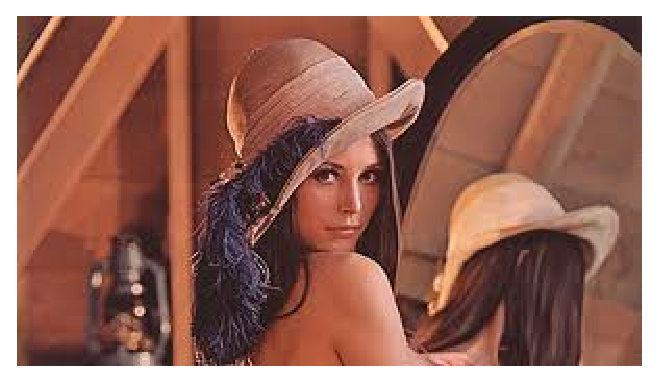
\includegraphics[scale=0.7]{Misc/TODO}
        \caption{A schematic phase diagram of a series of hole-doped cuprates}
        \label{Fig:1:UniversalCupratePhaseDiagram}
    \end{center}
\end{figure}
From the standpoint of conventional superconductivity, the first striking feature is the proximity of an antiferromagnetic phase to the superconducting region. Even without actual temperature labels, it becomes clear that if this was a phonon mediated superconductor, the pairing must be strong in order to overcome the strong spin-density wave scattering that results in the anitferromagnetic state.

Another interesting region, one that is not present in the pnictides, is that below the $T^*$ temperature scale on the underdoped side of the superconducting dome. In this region, an energy gap opens up in the excitation spectra but without any sign of the Meissner effect. This region is known as the \textit{pseudogap}. Some aspects of the pseudogap lead us to believe that it is closely related to the superconducting gap such as the fact that it shares the gap symmetry and is of a similar magnitude, and there have been proposals that the pseudogap is a precursor state to superconductivity TODO. However research involving the Bristol group has shown evidence that phase fluctuations rather than the pseudogap in particular are the neceesary precursors for the cuprate superconducting condition\cite{Rourke2011}.

\subsection{Anisotropic scattering}





\section{Cuprate doping determination}




% \chapter{Experimental Technique}


\section{De Haas-van Alphen torque oscillation}

In this section the phenomenon of \ac{dHvA} oscillations is described along with its measurement by the torque method. For decades, \ac{dHvA} has provided the principle method of characterising the Fermiology of a material with only relatively recent competition from techniques such as positron annihilation and \ac{ARPES} in particular. Whilst \ac{ARPES} can provide direct maps of Fermi surfaces within the Brillouin zone, \ac{dHvA} has some advantages such as the fact that it ignores surface effects such as crystal reconstruction, can determine cross-sectional areas with a relatively high resolution and also provides useful secondary measurements such as effective masses of the quasiparticle carriers.  Some disadvantages of the technique include the fact that \ac{dHvA} cannot locate particular cross-sectional orbits within the Brillouin zone (thus relies on secondary knowledge such as \ac{DFT} calculations) and also that the high magnetic fields could potentially affect the Fermi surface, for example by splitting the energy levels. Regardless \ac{dHvA} continues to be a reliable technique for Fermi surface characterisation. A more detailed comparison of all three techniques can be found in appendix~\ref{Appendix:FermilogyTechniques}.



\subsection{Theory}

\subsubsection{Overview}

For metals, the majority of the interesting physics occurs at the Fermi level and, provided Fermi liquid theory holds true, the electrons at the Fermi level can be modelled to a high degree of accuracy with the Sommerfeld model --- that is a Fermi gas of non-interacting electrons in an infinite box. When a magnetic field is applied, the electrons have their usual grid pattern distribution of plane wave k-vectors rearranged such that the electrons move around orbital and helical paths. These rearranged k-vectors form a set of concentric tubes, known as Landau tubes, whose cross-sectional area, $a$, perpedicular to the field is given by the Onsager relation:\footnote{Derivations of the Onsager relation are given in several textbooks including pg. 32 of Schoenberg\cite{Schoenberg1984} and pg. 272 of Ashcroft \& Mermin\cite{Ashcroft1976}.} 
%%
\begin{equation}
\label{Eqn:2:Onsager}
\textit{a}_{k_{\perp}} = (r + 1/2)\frac{2\pi e B}{\hbar}
\end{equation}
%%
where $r$ is a quantisation number that sets apart each tube. We can see from the relation that as $\vect{B}$ increases, so does the cross-sectional area of the tubes. As the magnetic field is ramped, successive tubes periodically pass the Fermi surface causing a spike in the \ac{DOS} at the Fermi level and also oscillations in the energy o the ssytem, $E$, which, for geometric reasons explained in the next section, are far stronger at the maximumal and minimal (extremal) areas of Fermi surface. Thermodynamic quantities such as magnetic susceptibility ($\chi = \partial E/\partial B$) and heat capacity ($C_{V} = \partial^2E/\partial T^2|_{V}$) or quantities that depend on the \ac{DOS} at the Fermi level such as electrical resistance all oscillate as the field is ramped. Oscillations in the susceptibility are known as \ac{dHvA} oscillations, oscillations in the resistivity are known as Shubnikov-de Haas oscillations.

 We can relate the `frequency' $F$ (measured in $tesla$\footnote{n.b. that it is \textit{tesla} and not \textit{tesla$^{-1}$} because, as we shall see later, the oscillations are actually periodic in $1/B$ and \textit{not} $B$ so their frequency counterpart is measured in \textit{tesla}.}) that the tubes pass the Fermi surface to the extremal Fermi surface area using the following application of the Onsager relation,
%%
\begin{equation}
\textit{a}_{k_{\perp}} = \frac{2\pi e }{\hbar}F
\end{equation}
%%
By varying the direction of the field we can obtain a series of maximal and minimal Fermi surface areas in a variety of orientations in order to build a profile of the Fermi surface topology and size. In practice, there are many possible variations that might fit the model based on areas of cross-sectional slices alone and so typically ab-initio \ac{DFT} calculations --- described in section~\ref{Sec:2:dft} --- are employed to provide a basis which can be tweaked based on the constraints from the measurements. 

A more detailed analysis of this process follows, beginning with an illustrative mathematical treatment for oscillations in the magnetisation.

\subsubsection{Oscillations in magnetisation}

We begin by calculating the degeneracy of the Landau tubes i.e. the number of electron states per tube. Because the states under a magnetic field are a one-to-one rearrangement of the states with no field, we can use the Sommerfeld number of states per unit k-space ($V/4\pi^3$) to determine the degeneracy. From the Onsager relation (eqn.\ref{Eqn:2:Onsager}) we see that the additional area for successive tubes is $\Delta a_{k_{\perp}}  = 2\pi e B/\hbar$ which we can convert to a volume by integrating over $k_{\perp}$. This gives a degeneracy per tube therefore of,

\begin{equation}
D_{\textrm{tube}} = d k_{\perp}\left(\frac{2\pi e B}{\hbar}\right)\left(\frac{V}{4 \pi^3}\right) = \frac{eBVdk_{\perp}}{\hbar 2\pi^2}
\end{equation}

We continue by writing an expression for the energy of the system, $E$ by summing the energies of the states that lie beneath the cross-sectional area defined by the Fermi surface ($a_{k_\perp F}$) for a given $k_\perp$. To do this, we use the Onsager equation to determine $R_\perp$ --- the number of Landau tubes below the Fermi surface at this cross-sectional slice. We then multiply this by the degeneracy of the tubes, $D$ and the energy for states on that particular Landau tube, $\epsilon_r$,
%%
\begin{equation}
\label{Eqn:2:OscillateE}
E = D\sum_{r}^{R_\perp}\epsilon_r = \frac{eBVdk_\perp}{\hbar 2 \pi^2}\sum_{r}^{R_\perp}\epsilon_r
\end{equation}
 where,
\begin{equation}
R_\perp = \textrm{floor}\left[\frac{a_{k_\perp F}\hbar}{2\pi e B} - \frac{1}{2}\right]
\end{equation}
%%
To complete the above equation, we need an expression for the energies of each of the Landau tubes. The procedure for the free electron case is to insert the canonical momentum (i.e momentum of a free electron in a magnetic field) into the non-interacting Schr\"odinger equation and solve to obtain the following eigenvalues for the energies on the Landau tubes. Full derivations can be found in several textbooks\footnote{See for examples pg. 32ff. in Schoenberg\cite{Schoenberg1984} or pg. 148ff. in Blundell\cite{Blundell2001}.} and so will  not be repeated here. Below is the expression for the energy eigenvalues,
%%
\begin{equation}
\epsilon_r=(r+1/2) \hbar \omega_c + \frac{\hbar^2 k^2}{2m_0}
\end{equation}
%%
where,
%%
\begin{equation}
\omega_c = \frac{eB}{m_0}
\end{equation}
%%
and is known as the \textit{cyclotron frequency}. The summation term in equation\ref{Eqn:2:OscillateE} can now be written,
%%
\begin{align*}
\sum_r^{R_\perp}\epsilon_r &= \sum_r^{R_\perp}\left( (r+1/2) \hbar \omega_c + \frac{\hbar^2 k^2}{2m_0} \right) \\
    &= \frac{\hbar eB}{m_0}\sum_r^{R_\perp}r + \frac{\hbar eB}{2m_0}\sum_r^{R_\perp}1 + \frac{\hbar^2 k^2}{2m_0}\sum_r^{R_\perp}1 \\
    &= \frac{\hbar eB}{2 m_0} R_\perp(R_\perp + 1) + \frac{\hbar eB}{2m_0}R_\perp + \frac{\hbar^2 k^2}{2m_0}R_\perp \\
    &= \frac{\hbar eB}{2m_0}R_\perp^2 + \left(\frac{\hbar eB}{m_0} + \frac{\hbar^2 k^2}{2m_0}\right)R_\perp
\end{align*}
%%
which can be expanded out and finally substituted back into equation\ref{Eqn:2:OscillateE} to finally obtain,
%%
\begin{equation}
\label{Eqn:2:OscIllustration}
E = \frac{eB^2Vdk_\perp}{4\pi^2m_0}\left[e R_\perp^2 + \left(2e + \frac{\hbar k^2}{B}\right)R_\perp\right]
\end{equation}
%%
Key to the above relation is that, although $R_\perp$ is inversely proprtional to $B$, it remains discrete. This gives rise to the saw-tooth like function shown in \fig\ref{Fig:2:EnergyOscillations} for some typical experimental parameters. Also plotted is the fuction against $1/B$ where we can clearly see that the oscillations are periodic in inverse field hence the frequency being measured in tesla$^{-1}$.
%%
\begin{figure}[htbp]
    \begin{center}
        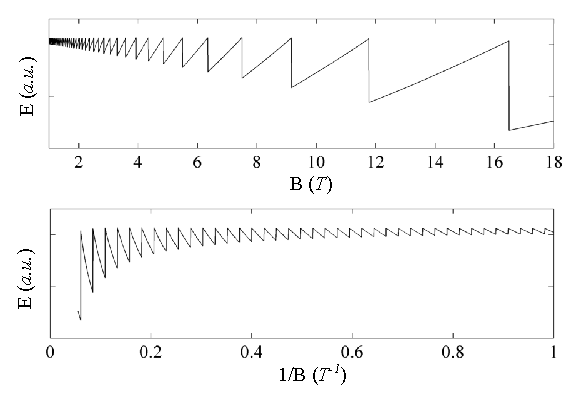
\includegraphics[scale=0.9]{Chapter2-ExperimentalTechnique/Figures/TheoreticalOscillations/TheoreticalOscillations}
        \caption{Theoretical energy oscillations for a Fermi surface orbit which is 5\% of a \unit[5]{\AA} cubic Brillouin zone between \unit[1--18]{T}. Kinetic energy term is taken to be for an electron at a level half the size of the Fermi surface.}
        \label{Fig:2:EnergyOscillations}
    \end{center}
\end{figure}

The above is not a rigourous derivation but is nonetheless illustrative of the origin of the oscillation in the system energy and how any thermodynamic value which depends on the energy of the system oscillates as a function of field. To continue we need to include correction factors to the oscillation amplitude due to finite electron scattering rates ($A_D$), temperature ($A_T$), Zeeman splitting of spins ($A_s$), doping ($A_{\textrm{dop}}$), mosaicity ($A_{\textrm{mos}}$), warping of the Fermi surface ($A_{\textrm{warp}}$) as well as adjustments due to the fact that the parameter measured was torque of the sample in a field and not the energy or magnetisation directly ($A_{\Gamma}$). For this, we turn to a more solid foundation that was put forward by Lifschitz and Kosevitch and presented by Schoenberg.

\subsubsection{\acl{LK} equation}

The derivation for the full expression for the Landau thermodynamic potential, $\Omega$\footnote{Formally defined as the energy in a open system that is in thermal contact with its surroundings}, begins in a similar way to the previous illustrative example but frames the sawtooth-like function above as a more mathematically manageable Fourier decomposition which also conveniently makes the technique highly amenable to Fourier analysis. For this reason the equation below features higher harmonics which are denoted with the identifier $p$.
%%
\begin{equation}
\Omega = \left(\frac{e}{2\pi\hbar}\right)^{\frac{3}{2}}\frac{e\hbar B^{\frac{5}{2}}}{m_0 \pi^2}\left| \frac{\partial^2 a_{\textrm{ext}}}{\partial k^2_\perp}\right|^{-\frac{1}{2}}\sum_{p=1}^{\infty}p^{-\frac{5}{2}}A\cos\left[2\pi\left(\frac{F}{B} - \gamma\right)\pm\frac{\pi}{4}\right]
\end{equation}
where,
\begin{equation}
A = A_T A_D A_s A_{\textrm{mos}} A_{\textrm{dop}} A_{\textrm{warp}} 
\end{equation}
The above equation and derivatives of it are known as the \ac{LK} equation. We no longer have the integral over $k_\perp$ and instead have the parameter $a_{\textrm{ext}}$ which is (one of) the extremal Fermi surface orbit area(s) perpendicular to a particular field direction. Only the extremal (i.e. the largest and smallest) magnetically induced orbits contribute significantly to oscillations in the system energy. The reason for this is that when performing the integral over $k_\perp$ to attain the \ac{LK} equation, $F$ varies as a function of $a_{k_\perp}$ and hence as a function of $k_\perp$. This leads to a blurring of the phase in the cosine term for a given $B$ which reduces the overall amplitude significantly. Regions where $dF/dk_\perp$ is small (i.e. turning points) therefore have more orbits across the integration that are closely in phase and are therfore stronger

TODO

The modifications to the \ac{LK} equation listed towards the end of the previous section can be manifest by convolving an appropriate phase distribution function with the cosine oscillatory term. It can be shown\footnote{See for example, Schoenberg pg 57--59.\cite{Schoenberg1984}} that this convolution results in a relatively simple multiplication factor, hence the various $A$ factors listed in the equation.


\subsubsection{Extracting the effective mass from the temperature}

The temperature effects on the \ac{LK} equation are One possible way to introduce temperature effects is to consider that the Fermi energy $\mu$ may be smeared according to the Fermi distribution $f(\epsilon) = 1/(1+\exp((\epsilon-\mu)/kT))$.





Originally \ac{dHvA} measurements were used to measure the Fermi surfaces of elemental metals and so the initial assumption of a free-electron gas is justified based on the fact that elemental metals have a Fermi surface and are considered materials that adhere to Fermi liquid theory. The fact that oscillations have been observed in cuprates and pnictides which have demonstrated non-Fermi liquid behaviour is therefore remarkable and moreover implies the presence of a Fermi surface, at least in the prescence of a strong magnetic field.



\subsection{Mapping the Fermi surface}

\subsubsection{Background removal}
% TODO: Removal of background should not be done against 1/B as a rule.
% Include investigation as to low frequency peak
Previous standard practice was to remove a background polynomial fitted to the field or inverse field from the raw data before taking the FFT. \Fig\ref{Fig:2:BackgroundSubtraction} shows raw torque data taken over a range of angles\footnote{See section\ref{Sec:3:AngleDependentMeasurements} for full details} and a strong $H^2$ component can be observed as a result of the $R_{\Gamma}$ term in equation\ref{}. Subtracting a second order polynomial fitted to the \textit{inverse} field leaves a large artificial angle-dependant oscillation in $1/H$ in the residual which may be misconstrued as a signal from a low frequency Fermi surface orbit. For this reason it is recommended to subtract a second order polynomial fitted to field rather than inverse field for torque measurements.
\begin{figure}[h!]
    \begin{center}
        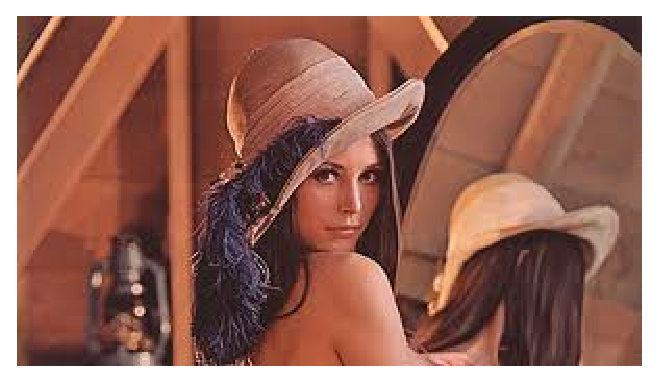
\includegraphics[scale=0.7]{Misc/TODO}
        \caption{Left panel shows the angle dependance of the raw torque signal  clearly showing a positive $H^2$ component for $\theta>0$ and a $-H^2$ component for $\theta<0$. Centre panel shows the FFT vs. angle for data with the 2nd order polynomial fitted to $1/H$ removed. A strong angle dependant peak at low frequency is seen. Right panel shows the same data but with a second order polynomial fitted to $H$ removed.}
        \label{Fig:2:BackgroundSubstraction}
    \end{center}
\end{figure}



\subsection{Measuring the spin mass}

\subsection{Measuring the band mass}

\subsubsection{Basic LK formula fitting}

Of all the damping terms in the \LK equation, only $R_T$ has any kind of temperature dependancy. This term also features the effective mass. By measuring oscillations at a fixed angle but with varying temperatures, the effective mass can be determined. However there is a difficulty in that in-order to observe oscillations, it is necessary to sweep the magnetic field, and many other damping terms have a field dependancy. To the first approximation, an inversely averaged applied field can be used in the \LK equation provided that the field sweep range is small. However there are a couple of techniques that were employed in order to overcome this shortcoming.

\subsubsection{Retrofitting ansatz LK formulae}
\label{Sec:2:LKRetrofitting}

One of the primary field-dependant contributions to the oscillation amplitude is the Dingle term scattering (equation \ref{Eqn:2:DingleTermOscillationAmp}). This has an exponential dependance with temperature. The Dingle factor, $\alpha$, can be determined by fitting a simplified version of equation \ref{Eqn:2:OscillationAmp} to oscillations which have been filtered to reduce the number of fitting parameters. Once we have the Dingle term, a series of ansatz data TODO...




\subsubsection{`Microfitting' the LK formula}
\label{Sec:2:LKMicrofitting}

\subsection{Method}

Two separate arcs of extremal area were mapped for the angle dependent measurements. One goes along the arc from $B\parallel c$ towards the $a$ axis, the other goes along the arc from $B\parallel c$ towards the $110$ direction. The former we call the $100$ arc, the latter the $110$ arc. In fact, measurements start further back beyond the $B\parallel c$ direction in order to ensure that the minima was reached and to correctly align the crystal as described below.

\subsubsection{Angle correction}
    \label{Sec:2:AngleCorrection}

To perform angle dependent measurements, we need to first of all measure accurately the angle between subsequent measurements and second we need to determine the angle of the field compared to the basel planes of the crystal. A further problem is that of aligning the basel plane with respect to the arc of rotation, something that is discussed, briefly here, but in more detail in the results in section~\ref{Sec:3:DFTShifts}.

In order to tackle the first problem, the sample platform is subject to a weak oscillating magnetic field from a large coil mounted inside of the yellow cryostat.\footnote{An upper bound on the strength is $\sim$\unit[500]{Gauss}, based on \unit[2.2]{mV} after $\times100$ amplification measured across a coil of $\sim140$ turns with an average area of \unit[3.36]{$mm^2$} per loop} A voltage is induced in a smaller coil which is mounted on the rotating portion of the sample platform\footnote{In fact there are two small coils, each perpendicular to one another although only one is measured at a time} which is proportional to the sine of the angle between the coil and the AC field. By monitoring this voltage, accurate determination of the angle between the sample platform and the field can be made and therefore the angle between subsequent measurements.

The correct angle between the large DC field and the crystal planes in the sample were determined using a post-measurement correction. Since the frequency of the quantum oscillations are field dependent with turning points at the $H\parallel [001]$ direction for approximately two dimensional samples, an even termed polynomial up to fourth order was fitted to the peaks. From the minima of the fits an angular offset was obtained which gave the final correction to the above coil measurements.

The basel angle was aligned on the cantilever by eye. This was coupled with XRD measurements which determined how the visual features corresponded to the crystal axes. This leads to an estimated error in basel plane alignment of around \unit[5]{\%} although we found evidence for greater misalignment in one case, detailed in the results.

\subsubsection{Temperature correction}
    \label{Sec:2:TemepratureCorrection}

Effective mass measurements on particular extremal orbits rely on accurate temperature determination at all stages of the field sweep. On the Yellow magnet system, temperature from base of $\approx$\unit[0.3]{K} to $\approx$\unit[2]{K} is controlled by adjusting the He$^3$ sorbtion pump temperature and can be considered to be independant of field effect since the thermometer regulating the sorb temperature is outside of the strong field core. However if we consider \fig\ref{Fig:2:TemperatureCorrection}, it is evident that there are magnetic field effects on the RuOx, which is mounted in the base of the magnet but thermally linked with the sample, and the Cernox thermometer that sits on the sample stage.
\begin{figure}[htbp]
    \begin{center}
        \includegraphics[scale=0.9]{Chapter3-dHvABaFe2P2/Figures/Mass/TemperatureCorrection/TemperatureCorrection}
        \caption{Some example temperature readings (squares) set using the sorbtion pump heater. Also shown are corrections (circles) by interpolating to known values. RuOx thermometer is shown in blue, Cernox stage thermometer is shown in red. Second order polynomial fits to the data are shown as lines extrapolated to zero to get a rough estimate of the zero field temperature value.}
        \label{Fig:2:TemperatureCorrection}
    \end{center}
\end{figure}
Readings from both thermometers were taken with field sweeps from zero field up to \unit[18]{T} at steady temperatures \unit[0.30]{K}, \unit[0.53]{K}, \unit[0.64]{K}, \unit[1.06]{K} and \unit[1.34]{K}. By interpolating between this data\footnote{Performed using multiquadric radial basis functions from the Scipy Python library.}, the two thermometers can be correctied to agree within $\sim$\unit[0.01]{K}. This interpolation is however limited to temepratures below approximately \unit[1.45]{K} as is shown in the figure for readings at around \unit[1.6]{K}. In these cases, the less reliable method of extrapolating the readings back to zero field using a second order polynomial fit are used as demonstrated with the solid lines in \fig\ref{Fig:2:TemperatureCorrection}. In these cases the temeprature is taken to be the mean of the two extrapolated values with the differences defining the error.


\subsection{Yellow Magnet}

dHvA Measurements were all performed in Bristol on the `Yellow Magnet' system which was built by Oxford and can nominally operate up to \unit[20]{t} with use of the lambda plate although more typically is operated up to \unit[18]{T}. The sample sites on a one axis rotator and angle is determined by one of two orthogonal pick-up coils mounted on the sample stage weak, oscillating magnetic, field in




\section{Measuring charge transport}

\subsection{Fermi liquid theory}

\subsection{Hall effect}

\subsection{Magnetoresistance}

\subsection{Six probe technique}

\subsection{Sample size determination}




\setcounter{chapter}{2}
\chapter{dHvA measurements on \BaFeP}


\section{The \BaFePAs series}

The \BaFePAs series is one of many that stem from the parent compount \BaFeAs, although unlike the electron doped \BaCoFeAs and the hole doped \BaKFeAs series, the \BaFePAs progression is entirely isovalent meaning that the changes affected due to the P substitution are due to structure and chemical pressure rather than additional charge carriers. Nonetheless, superconductivity occurs with a very similar phase diagram as with the charge-doped examples in the same `$122$' family of iron-pnictide materials.\footnote{See for example \Fig1 in ref.\cite{Paglione2010}}

At $x=0$ the \BaFePAs series begins at \BaFeAs, a compound which becomes antiferromagnetic at around \unit[138]{K}, and moves with increasing $x$ towards \BaFeP which is metallic to low temperatures. Neither end members are superconducting, however as As is substituted for P, the low temperature antiferromagnetic state decays, giving way to superconductivity which kicks in at approximately $x=0.18$ and increases to the optimal substitution of $x=0.31$. Superconductivity then decreases until it gives way to a paramagnetic ground state at around $x=0.71$. \Fig\ref{Fig:3:PhaseDiagram} shows the phase diagram adapated from ref. \cite{Nakai2010a} as determined by resistivity measurements. 
\begin{figure}
    \begin{center}
        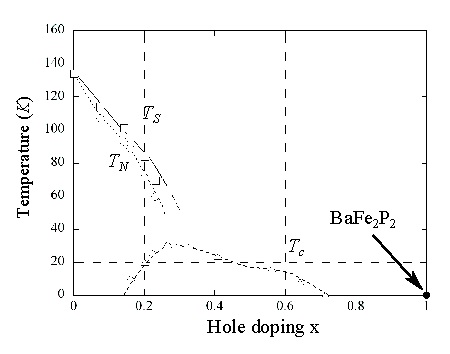
\includegraphics[scale=1.0]{Chapter3-dHvABaFe2P2/Figures/BaFe2P2Series/PhaseDiagram/PhaseDiagram}
        \caption{Phase diagram adapted from ref \cite{Nakai2010a} measured by resistivity. $T_s$, $T_N$ and $T_c$ are the structural transition, the antiferromagnetic transition and the superconducting transition temperatures respectively.}
        \label{Fig:3:PhaseDiagram}
    \end{center}
\end{figure}
Also detailed in the phase diagram is the structural transition which occurs as the tetragonal $I4/mmm$ cell moves to an orthorhombic cell as it passes below the line marked $T_s$. This is a feature which is common to many of the `$122$' pnictide materials.

 The progression along the series is isovalent since P and As are in the same periodic group -- group $V$. The net effect of the substitution is to apply an increasing chemical pressure as $x$ moves towards $1$. Several reports show that applying \textit{physical} pressure to \BaFeAs results in a similar phase diagram with an antiferromagnetic phase and superconductivity up to $\sim$\unit[30]{K}\cite{Yamazaki2010,Colombier2009,Alireza2009} with Klintberg \textit{et al.}\cite{Klintberg2010} presenting a direct comparison between the two types of pressure. As pressure is applied, the unit cell $a$ axis shrinks slightly less than the $c$ axis ($\sim3\%$ c.f. $\sim4.5\%$ respectively). Interestingly the $c$ axis shrinking largely occurs in the Fe-Pnictide plane leading to some theories of the superconductivity emerging from the tetrahedral bond angle between the Fe and the pnictigen. %TODO: ref
\begin{figure}
    \begin{center}
        \includegraphics[scale=1.0]{Chapter3-dHvABaFe2P2/Figures/BaFe2P2Series/UnitCell/UnitCell}
        \caption{The tetragonal unit cell of the 122 \BaFePAs series.}
        \label{Fig:3:UnitCell}
    \end{center}
\end{figure}


The \BaFePAs series from a substitution of $x=0.41$--$1.0$ has been previously measured by members of the group at Bristol using dHvA oscillations\cite{Shishido2010}. As suggested in the Shishido reference, since dHvA has been observed across such a large range of substitutions, it implies that the material is not prone to disorder as is the case in many charge doped series (TODO ref) making the series an excellant candidate for dHvA studies. The Fermi surfaces have been characterised for x ranging from $0.41$ to $1$ for electron sheets only but have clearly shown that the DFT calculations consistently overestimate the size of the surfaces. Moreover, dHvA measurements on the material with $x=0.63$ have been performed where one of the hole surface extrema was observed\cite{Analytis2010c} however DFT calculations as well as comparisons with \SrFeP\cite{Analytis2009} give evidence for a second hole Fermi surface for materials towards the P end of the series, (towards the As end of the series, there appears this second hole and a \textit{third} hole surface -- a pinched off, 3D surface around the $\Gamma$ point). If the electron Fermi surfaces are oversized in the DFT calculations, then the hole Fermi surface volumes should also be oversized in order to remain compensated (electrically neutral). What is not clear though is whether the \textit{shapes} of the hole pockets are also altered in the compounds leading to \BaFeP. DFT calculations show the larger of the hole pockets in particular undergoing significant geometric changes, specifically in that it becomes much more three dimensional as P substitution becomes more complete. The Fermi surface of the opposite end-member, \BaFeAs, has been fully characterised by previous ARPES measurements\cite{Kondo2010a} and dHvA\cite{Terashima2011, Analytis2010b}. Coupled with a full characterisation of the fermiology of \BaFeP, this data can be used to interpolate Fermiology of the hole pockets between end members thus completing the partial determination of the Fermi surfaces of the intermediary compounds.

The ARPES measurements of the Fermi surface of \BaFeAs below the N\'eel temperature concluded that despite some $k_z$ dispersion in the Fermi surfaces, there is adequate nesting to form the antiferromagnetic state. Ab-initio DFT calculations\cite{Shishido2010} of the paramagnetic state have shown the $k_z$ dispersion increasing with increasing P, with the outer hole pockets becoming more three-dimensional through the progression providing the partial nesting conditions necessary for pair forming SDW fluctuations described in section\ref{Sec:1:Nesting}. One caveat is that these calculations do not take into account the structural changes below $T_s$, another caveat is that they do not consider Fermi surface reconstruction due to the observed commensurate antiferromagnetic order. To fully settle the issue of the nature of the nesting in the sueprconducting state a good experimental determination of the Fermi surfaces of the series is necessary, a good guide to which can be obtained from study of the end-members.

This thesis presents data which details the full Fermi surface of \BaFeP including an elucidation of the shape of the 3D outer hole surface. Partial nesting is detailed between the outer hole surface and the inner electron surface with $q=(\pi, \pi, \pi/2)$ meaning the phenomenum persists through to the end member of the series. Also presented are effective mass measurements which show relatively small mass enhancements implying weak carrier correlations.



\section{X-Ray Diffraction}
    \label{Sec:3:XrayDiffraction}

The crystalline axes of the sample were determined on a Kappa Apex II single crystal diffractometer with the help of Mairi Haddow. The sample was mounted on a glass rod using vacuum grease during the measurements.
%%
\begin{figure}[h!]
    \begin{center}
        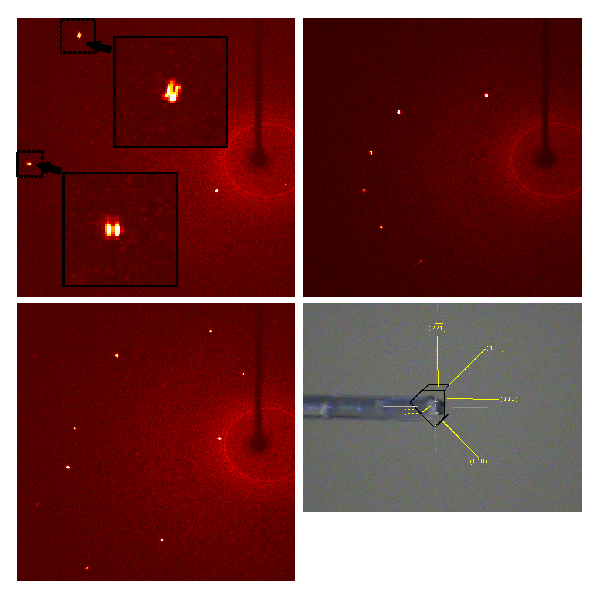
\includegraphics[scale=0.7]{Chapter3-dHvABaFe2P2/Figures/Xrays/XRayDiffraction/XrayDiffraction}
        \caption{Top left, top right and bottom left show example diffraction patterns of the \BaFeP sampple. Top-left shows a zoomed portion of doubled peaks indicating that there may potentially be a misalignment within the crystal. Bottom right shows the labeled crystal axes superimposed on the sample which is mounted on a glass rod.}
        \label{Fig:3:XRayDiffraction}
    \end{center}
\end{figure}

Table~\ref{Table:3:LatticeParams} shows the lattice parameters as determined by the x-ray measurements.
%%
\medskip
%% 
\begin{center}
    \begin{tabular}[h!]{llr}
\toprule
Source  &  $a$ (\AA) & $c$ (\AA) \\
\midrule
X-ray   & 3.82  & 12.38 \\
Mewis et al.\cite{Mewis1980} & 3.84 & 12.44 \\
Rotter et al.\cite{Rotter2010} & 3.84 & 12.42 \\
\bottomrule
    \label{Table:3:LatticeParams}
    \end{tabular}
\end{center}




\section{Angle dependent measurements}
    \label{Sec:3:AngleDependentMeasurements}

\subsection{Preliminary measurements}

Preliminary measurements showed very strong dHvA oscillations which begin at relatively low field.  An example of the raw data can be seen in \fig~\ref{Fig:3:RawOscillations}. Since is is not clear from the raw oscillations where the oscillations begin, Fourier transforms were taken with small field windows -- the interval where a clear signal is present marks the onset of oscillations. A FFT of the data between $6\unit{T}$ and $7\unit{T}$ is shown in the inset of the figure. This clearly shows the electron peaks at $1370\unit{T}$, $2175\unit{T}$ and $2343\unit{T}$, whereas below $6\unit{T}$ there was no appreciable signal. For subsequent measurements the field was ramped between $6\unit{T}$ and the dafe maximum of $18\unit{T}$ unless otherwise stated.

\begin{figure}[h!]
    \begin{center}
        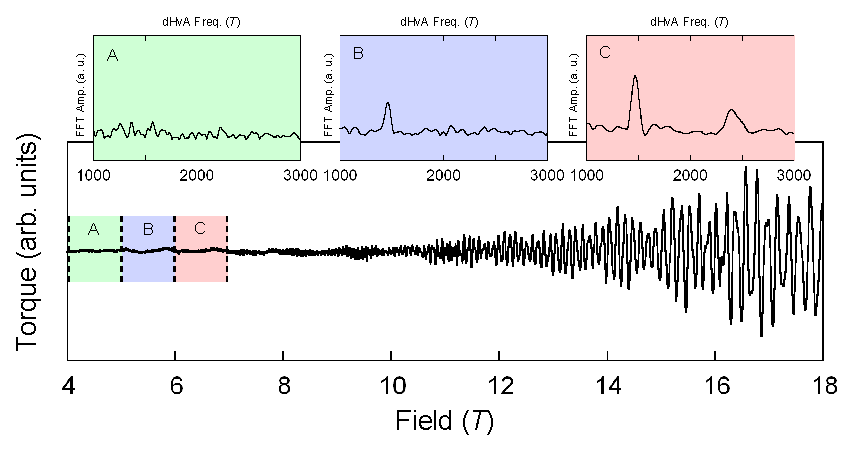
\includegraphics[scale=0.7]{Chapter3-dHvABaFe2P2/Figures/AngleDepMeasurements/RawOscillations/RawOscillations}
        \caption{An example of the torque data taken with field aligned at $9\degree$ from the $[001]$ direction. Inset shows a FFT of the data between $6\unit{T}$ and $8\unit{T}$}
        \label{Fig:3:RawOscillations}
    \end{center}
\end{figure}


 \Fig~\ref{Fig:3:RawOscillationSamples} shows some example Fourier transforms of data taken at various sweep rates. Since there is little difference between the sweeps at $0.05\unit{T/min.}$ and $0.1\unit{T/min.}$, subsequent sweeps were performed at $0.1\unit{T/min.}$.

\begin{figure}[h!]
    \begin{center}
        \includegraphics[scale=0.7]{Chapter3-dHvABaFe2P2/Figures/AngleDepMeasurements/SweepRateComparison/SweepRateComparison}
        \caption{FFTs showing the peak from the smaller branch of band $3$ shifted arbitrarily for comparison with the $B$ field at $10\degree$ from $[001]$ int the $[110]$ direction. Sweeps were performed at, A: $0.05\unit{T/min.}$, B: $0.1\unit{T/min.}$ and C: $0.2\unit{T/min.}$}
        \label{Fig:3:ComparisonSweepRates}
    \end{center}
\end{figure}

Measurements were taken at one degree intervals from the $B || c$-axis ($[001]$) down to $B || [100]$ and from $B || c$-axis down to $B || [110]$. \Fig~\ref{Fig:3:FFTExamples} shows three example FFTs which show all the bands identified the next section. They also show first and second harmonics\footnote{Third harmonics were also identified in other FFTs, these are marked in \fig~\ref{Fig:3:AngleSweepMeasured}.}.

\begin{figure}[h!]
    \begin{center}
        %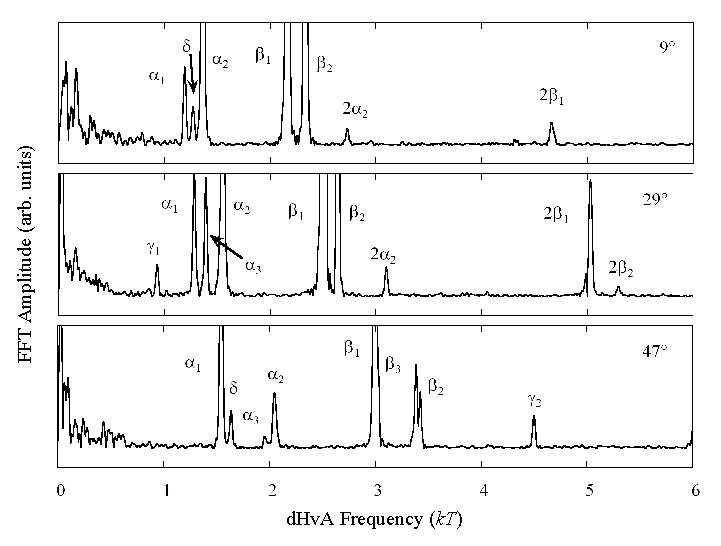
\includegraphics[scale=0.7]{Chapter3-dHvABaFe2P2/Figures/AngleDepMeasurements/FFTExamples/FFTExamples}
        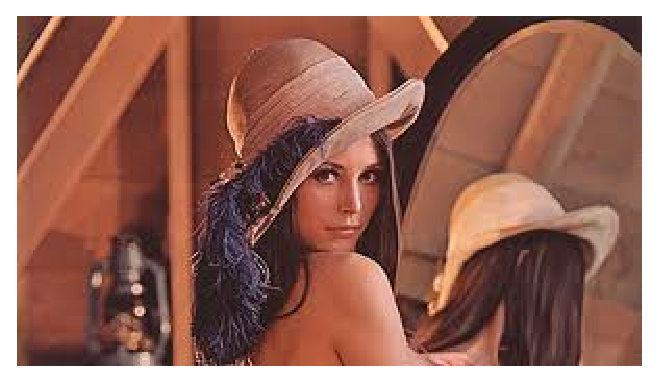
\includegraphics[scale=0.7]{Misc/TODO}
        \caption{}
        \label{Fig:3:FFTExamples}
    \end{center}
\end{figure}

The highlighted, low frequency region in \fig~\ref{Fig:3:FFTExamples} shows some Fourier weight which contains low-frequency noise and background from the cantilever but, according to later analysis, likely contains signal from the minimum of band $1$.


TODO: Example FFT
TODO: Low frequency noise investigation


\subsection{Mapping the Fermi surface with DFT calculations}
    \label{Sec:3:MappingFermiSurfaceDFTCalulations}

DFT calculations were performed using WIEN2k~\cite{Blaha2001} using the Generalised Gradient Approximation (GGA). This code was then processed using MATLAB code\footnote{Main body of code developed by Dr. Ed Yelland, School of Physics \& Astronomy, room 162, University of St Andrews, North Haugh, St Andrews KY16 9SS} to render a simulation of angle dependant dHvA measurements which is shown in \fig~\ref{Fig:3:ComparisonRotationPlotUnshiftedDFT}. 


\begin{figure}[h!]
    \begin{center}
        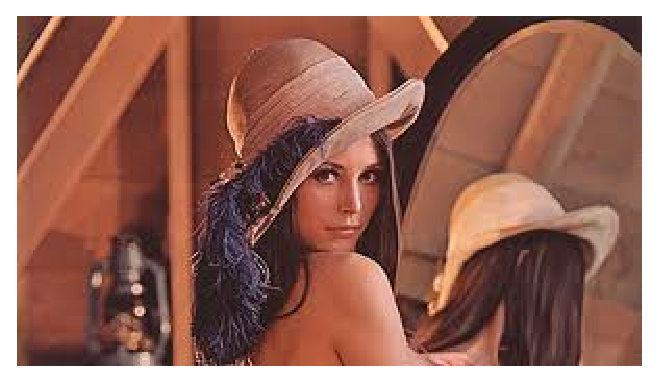
\includegraphics[scale=0.7]{Misc/TODO}
        \caption{dHvA frequencies nultipled by angle of the $B$ field. Solid lines are DFT calculations, open circles are measured data. $B$ field directed along (a) $[001]\rightarrow[100]$ and (b) $[001]\rightarrow[110]$.}
        \label{Fig:3:ComparisonRotationPlotUnshiftedDFT}
    \end{center}
\end{figure}

For the $[110]$ direction it became apparent from the fact that the DFT and the measured curves were qualitatively different that the field was not perfectly aligned with the $[110]$ axis of the sample. By assuming that the measurements were taken from the $c$-axis direction down to a vector rotated $10\deg$ within the $ab$-plane from the $[110]$ direction, the DFT data matches much better. This is within the estimated error for alignment from the microscope images.


\subsubsection{Rigidly shifting the calculated DFT energies}

As is shown in \fig~\ref{Fig:3:ComparisonRotationPlotUnshiftedDFT}, the rotation plots from the DFT calculations match up qualitatively with the data but do not match up quantitatively -- the electron bands overestimating the size of the measured extremal orbits by around TODO and the hole orbits overestimating the extremal orbits by around TODO. 

\begin{figure}[h!]
    \begin{center}
        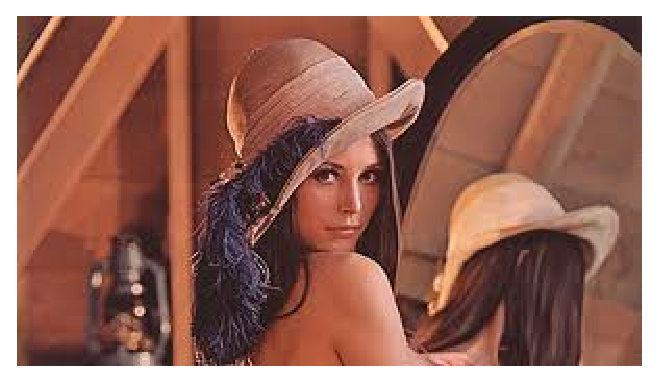
\includegraphics[scale=0.7]{Misc/TODO}
        \caption{dHvA frequencies multipled by the cosine of the angle of the $B$ field. Solid lines are rigidly shifted DFT calculations, open circles are measured data. $B$ field directed along (a) $[001]\rightarrow[100]$ and (b) $[001]\rightarrow[110]$.}
        \label{Fig:3:ComparisonRotationPlotMeasuredShiftedDFT}
    \end{center}
\end{figure}

In order to obtain the correct shape of Fermi surface, the DFT calculations need to be tweaked. One technique is to apply small band-specific rigid energy shifts, which, in most cases is enough to bring the DFT in line with the experimental data. \fig~\ref{Fig:3:ComparisonRotationPlotMeasuredShiftedDFT} shows the rotation plots which rotate towards both the 100 and 110 directions along with appropriately shifted calculations. Table~\ref{Table:3:EnergyShifts} lists those energy shifts.

\medskip

\begin{center}
    \begin{tabular}[h!]{llr}
\toprule
Band    & \multicolumn{2}{l}{Energy Shift (\unit{Ry})} \\
\midrule
1       &       & -0.0083      \\
2       & Wide  & 0.0          \\
        & Narrow & -0.0038     \\
3       &       & 0.0043       \\
4       &       & 0.0050        \\
\bottomrule
    \label{Table:3:EnergyShifts}
    \end{tabular}
\end{center}

Band $2$ in this case has two separate shifts specified in two different regions of the Brillouin zone. The rotation plot for the wider orbit located at the edge of the Brillouin zone was calculated with no energy shift and the narrow part of the Fermi surface around the $\Gamma$ point was calculated with a shift of $0.0038\unit{Ry}$. This provides a reasonable match for the rotation plot where we can apply the shift to the two regions discretely, however is proves problematic when we wish to study intermediate areas since it is not clear how the Fermi surface varies between the two regions.

\subsubsection{Shifting the DFT calculations proptional to orbital character}
\label{Sec:ShiftingDFTPropToOrbitalCharacter}

\Fig~\ref{Fig:3:Band2DCharacter} shows the strength of various d-orbital band characters taken on a 110 cut through the \BaFeP Brillouin zone with the band $2$ Fermi surface superimposed. Band characters for the other bands can be found in Appendix~\ref{TODO}.
%%
\begin{figure}[h!]
    \begin{center}
        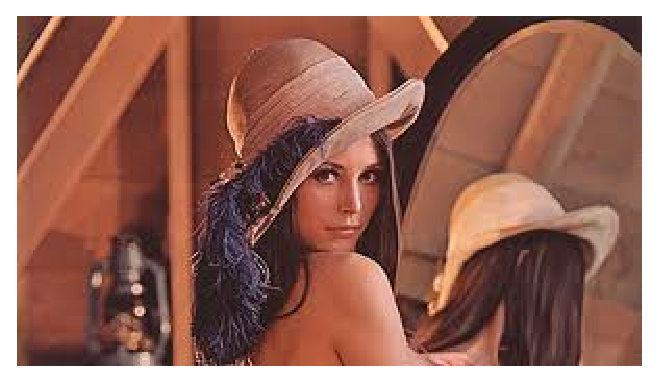
\includegraphics[scale=0.7]{Misc/TODO}
        \caption{Partial $d$-orbital character of the hole band $2$ across slices in the 110 direction. Solid lines show the Fermi surface in the plane.}
        \label{Fig:3:Band2DCharacter}
    \end{center}
\end{figure}
%%
\begin{figure}[h!]
    \begin{center}
        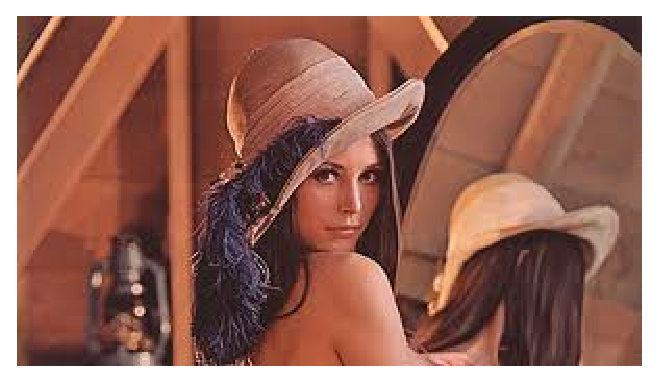
\includegraphics[scale=0.7]{Misc/TODO}
        \caption{Partial $d$-orbital characters of the hole band $2$ along the Fermi surface in the 110 slice vs. \kz}
        \label{Fig:3:Band2DCharacterVsKz}
    \end{center}
\end{figure}

Band $2$ has very little \Dxy and \DxTwoyTwo character close to the Fermi level but shows a significant amount of \DzTwo character at the wide region of the Fermi surface and \DxzDyz character at the narrow region. \Fig~\ref{Fig:3:Band2DCharacterVsKz} shows the orbital character for each of the $d$-orbitals as a function of \kz along the Fermi surface. Evidently, energy shifts could be applied which are scaled to either the \DzTwo and \DxzDyz orbital character in order that we obtain a smooth energy shift transition between the narrow and wide regions discussed previously.

Energy shifts were applied across the full $3$d Brillouin zone for band $2$ using the following two scalings,
%%
\begin{align*}
\textrm{\DzTwo:}\quad \Delta\epsilon &= 0.002 - 0.0052 (1 - (\epsilon - 0.033)/(0.2205 - 0.033)) \\
\textrm{\DxzDyz:}\quad \Delta\epsilon &= 0.002 - 0.0052 (\epsilon - 0.0946)/(0.3135 - 0.0946)
\end{align*}
%%
Note that these scalings ensure that the energy shift applied varies between $-0.0032\unit{Ry}$ and $0.002\unit{Ry}$ which are slightly different to the values applied when rigidly shifting the band. This is due to the fact that the Fermi surface area measured in one region is affected more and more by the size of the Fermi surface in the opposite region as the azimuthal angle gets higher and the calculated area deviates from the measured area. This is what results in the crossing of the calculated rotation plot with the measured rotation plot shown in the first panel of \fig~\ref{Fig:3:Band2DCharacterRigidComparison}. A rigid shift was therefore chosen which best lines up along the length of the curve -- one which will be slightly lower than if we were to match the plots exactly at the 001 direction.

\begin{figure}[h!]
    \begin{center}
        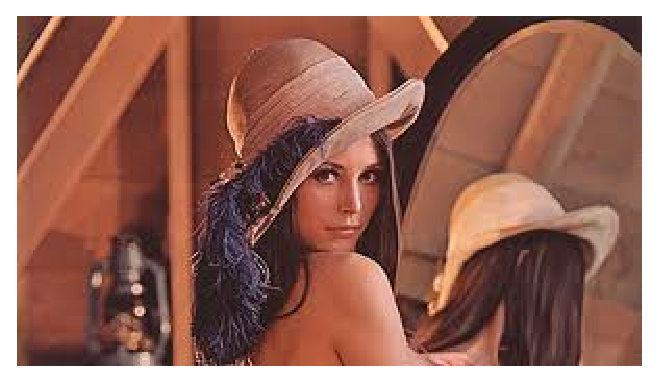
\includegraphics[scale=0.7]{Misc/TODO}
        \caption{dHvA frequencies for band 2 multipled by the cosine of the angle of the $B$ field. $B$ field directed along $[001]\rightarrow[110]$. Open circles are measured data, solid lines represent (a) rigidly shifted DFT calculations, (b) DFT calculations shifted proportional to \DzTwo orbital character, (c) DFT calculations shifted proportional to \DxzDyz orbital character.}
        \label{Fig:3:Band2DCharacterRigidComparison}
    \end{center}
\end{figure}

The second and third panels of \fig~\ref{Fig:3:Band2DCharacterRigidComparison} show the rotation plots calculated with the energy shifts applied proportional to \DzTwo and \DxzDyz orbital character respecitvely. We observe a much better alignment of the measured and calculated data for all angles.

Using the rigid energy shifts for bands $1$, $3$ and $4$ and using shifts scaled to \DzTwo orbital character for band $2$, as well as incorporating the corrections discussed in section~\ref{Sec:3:MappingFermiSurfaceDFTCalulations}, \fig~\ref{Fig:3:FinalRotPlot} shows the measured rotation plot for all bands along with corrected DFT data. \Fig~\ref{Fig:3:DFTCorrectedUnitCell} shows the unit cell for \BaFeP from the corrected DFT calculations.

\begin{figure}[h!]
    \begin{center}
        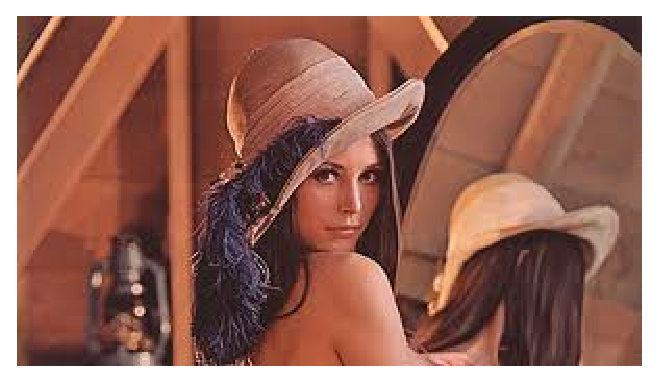
\includegraphics[scale=0.7]{Misc/TODO}
        \caption{dHvA frequencies for band 2 multipled by the cosine of the angle of the $B$ field. Open circles are measured data, solid lines represent DFT calculation shifted rigidly or scaled with the \DzTwo orbital character. $B$ field directed along (a) $[001]\rightarrow[110]$ and (b) $[001]\rightarrow[110]$.}
        \label{Fig:3:FinalRotPlot}
    \end{center}
\end{figure}
\begin{figure}[h!]
    \begin{center}
        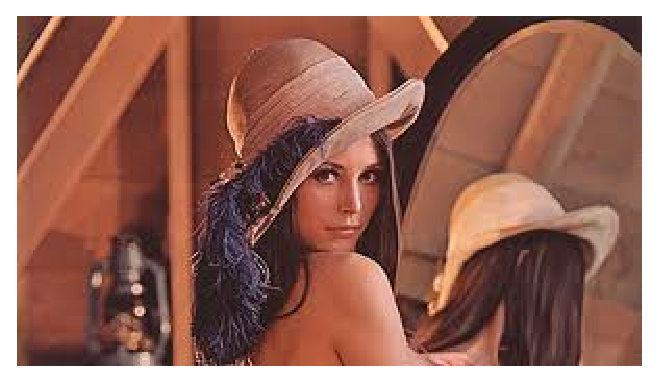
\includegraphics[scale=0.7]{Misc/TODO}
        \caption{Fermi surface in the first Brillouin of \BaFeP as determined by DFT calculations corrected by either rigid energy shifts (bands 1, 3, 4) or shifts proprtional to \DzTwo character (band 2)}
        \label{Fig:3:DFTCorrectedUnitCell}
    \end{center}
\end{figure}


\subsection{Susceptibility calculations}
\label{Sec:SubsceptibilityCalculation}



\section{Effective mass measurements}

\subsection{Temperature correction}

Effective mass measurements on particular extremal orbits rely on accurate temperature determination at all stages of the field sweep. On the Yellow magnet system, temperature from base of $\approx$\unit[0.3]{K} to $\approx$\unit[2]{K} is controlled by adjusting the He$^3$ sorbtion pump temperature and can be considered to be independant of field effect since the thermometer regulating the sorb temperature is outside of the strong field core. However if we consider \fig\ref{Fig:3:TemperatureCorrection}, it is evident that there are magnetic field effects on the RuOx, which is mounted in the base of the magnet but thermally linked with the sample, and the Cernox thermometer that sits on the sample stage.
\begin{figure}[htbp]
    \begin{center}
        \includegraphics[scale=0.9]{Chapter3-dHvABaFe2P2/Figures/Mass/TemperatureCorrection/TemperatureCorrection}
        \caption{Some example temperature readings (squares) set using the sorbtion pump heater. Also shown are corrections (circles) by interpolating to known values. RuOx thermometer is shown in blue, Cernox stage thermometer is shown in red. Second order polynomial fits to the data are shown as lines extrapolated to zero to get a rough estimate of the zero field temperature value.}
        \label{Fig:3:TemperatureCorrection}
    \end{center}
\end{figure}
Readings from both thermometers were taken with field sweeps from zero field up to \unit[18]{T} at steady temperatures \unit[0.30]{K}, \unit[0.53]{K}, \unit[0.64]{K}, \unit[1.06]{K} and \unit[1.34]{K}. By interpolating between this data\footnote{Performed using multiquadric radial basis functions from the Scipy Python library.}, the two thermometers can be correctied to agree within $\sim$\unit[0.01]{K}. This interpolation is however limited to temepratures below approximately \unit[1.45]{K} as is shown in the figure for readings at around \unit[1.6]{K}. In these cases, the less reliable method of extrapolating the readings back to zero field using a second order polynomial fit are used as demonstrated with the solid lines in \fig\ref{Fig:3:TemperatureCorrection}. In these cases the temeprature is taken to be the mean of the two extrapolated values with the differences defining the error.

\subsubsection{Basic LK formula fitting}

A series of field sweeps were taken with $H$ at \unit[12]{\degree}, \unit[28]{\degree} and \unit[46]{\degree} from $[001]$ in the $[110]$ direction. These were performed at a variety of temperatures from base ($\approx\unit[0.3]{K}$) to above \unit[2]{K}. \Fig~\ref{Fig:3:ExampleLKFits} shows the Fourier amplitude of various peaks as a function of temperature along with fits to equation~\ref{Eqn:2:TempTermOscillationAmp}. The field range for the FFT was was necessarily large enough that individual peaks did not overlap and also could be observed across a reasonable range of temperatures but also small enough so that the $B$ dependent Dingle factor did not play too large a role and so an average $B$ field can be assumed. The results from these fits are shown in table \ref{Table:3:RetroFittedLKResults} along with the fit ranges. All FFTs in the plot were taken over an interval of \unit[12--18]{T} with the exception of the $\gamma_2$ fit which was taken between \unit[16-18]{T} so as to attain an appreciable peak. The standard deviationw as calculated by randomly varying the temperature values by the estimated error (\unit[0.06]{K}) 1000 times and then taking the standard deviation of the fitted $m^*$ values.
%%
\begin{figure}[htbp]
    \begin{center}
        \includegraphics[scale=0.9]{Chapter3-dHvABaFe2P2/Figures/Mass/SimpleLKFits/SimpleLKFits}
        \caption{Fits to the temperature dependant part of the \LK formula. }
        \label{Fig:3:SimpleLKFits}
    \end{center}
\end{figure}
%%
Table \ref{Table:3:SimpleLKFitResults} also shows some results taken with a different field range. These fits give quite different values for the effective mass, indicating that the average field approximation is not a valid one.

\subsubsection{Retrofitting ansatz LK formulae}

The measurements presented in the previous section were further refined using the the ansatz LK formulae as described in section~\ref{Sec:2:LKRetrofitting}. \Fig~\ref{Fig:3:DingleTermExtractionFits} shows some sample fits used to extract the Dingle terms used in the ansatz fit functions.
%%
\begin{figure}[htbp]
    \begin{center}
        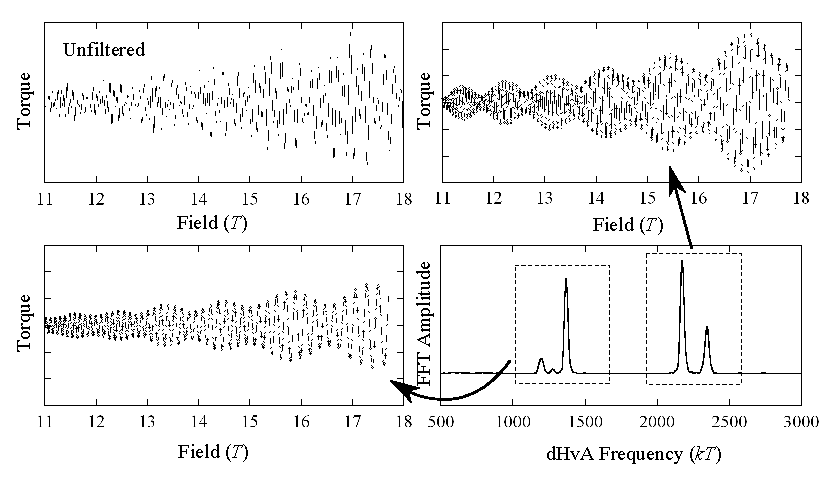
\includegraphics[scale=0.9]{Chapter3-dHvABaFe2P2/Figures/Mass/FittingDingleTerm/FittingDingleTerm}
        \caption{Top left panel shows torque data for data taken at \unit[12]{\degree} towards the $[110]$ direction at \unit[0.35]{K} with a polynomial background subtracted. Bottom right shows the FFT and the two filter windows to produce the filtered torque plots in the top right and bottom left. Filtered plots are fitted to extract the Dingle term for each frequency.}
        \label{Fig:3:DingleTermExtractionFits}
    \end{center}
\end{figure}
%%%%%
\begin{sidewaystable}
    \begin{center}
        \caption{Details of the calculations for the retrofitted masses. $m^*$ values are given in terms of electron rest mass, $m_e$}
{\small
        \begin{tabular}[htbp]{rrrrrrr}
\toprule
Angle	& Freq. (\unit[]{T})	& Label & $m^*$ & $m^*_{\textrm{retro}}$	& $\alpha$	& Field Lim. (\unit[]{T}) \\
\midrule
12	 & 1195	 & $\alpha_1$	 & 1.71(3)	& 1.75	& 58.681	& 12.0\\
12	 & 1195	 & $\alpha_1$	 & 1.49(2)	& 1.69	& 58.681	& 8.0\\
28	 & 1270	 & $\alpha_1$	 & 1.64(2)	& 1.68	& 59.602	& 12.0\\
46	 & 1540	 & $\alpha_1$	 & 1.86(3)	& 1.90	& 48.794	& 12.0\\
12	 & 1370	 & $\alpha_2$	 & 1.54(2)	& 1.58	& 45.989	& 12.0\\
28	 & 1526	 & $\alpha_2$	 & 1.69(2)	& 1.74	& 72.351	& 12.0\\
46	 & 2030	 & $\alpha_2$	 & 2.49(5)	& 2.56	& 61.058	& 12.0\\
28	 & 1370	 & $\alpha_3$	 & 1.85(3)	& 1.93	& 115.490	& 12.0\\
46	 & 1930	 & $\alpha_3$	 & 2.87(7)	& 3.04	& 149.390	& 12.0\\
12	 & 2176	 & $\beta_1$	 & 1.61(2)	& 1.65	& 51.119	& 12.0\\
12	 & 2353	 & $\beta_2$	 & 1.56(3)	& 1.62	& 102.360	& 12.0\\
12	 & 2353	 & $\beta_2$	 & 1.30(2)	& 1.87	& 102.360	& 6.0\\
28	 & 2603	 & $\beta_2$	 & 1.73(2)	& 1.76	& 34.082	& 12.0\\
46	 & 3335	 & $\beta_2$	 & 2.59(6)	& 2.69	& 94.572	& 12.0\\
28	 & 2472	 & $\beta_3$	 & 1.58(2)	& 1.61	& 48.807	& 12.0\\
46	 & 2972	 & $\beta_3$	 & 1.82(3)	& 1.86	& 40.033	& 12.0\\
46	 & 1320	 & $\gamma_1$	 & 2.13(5)	& 2.22	& 104.380	& 12.0\\
28	 & 920	 & $\gamma_1$	 & 2.19(3)	& 2.30	& 129.820	& 12.0\\
46	 & 4500	 & $\gamma_2$	 & 3.31(8)	& 3.32	& 91.057	& 16.0\\
12	 & 1285	 & $\delta_1$	 & 1.54(2)	& 1.64	& 173.000	& 12.0\\
28	 & 1370	 & $\delta_1$	 & 1.85(3)	& 1.93	& 115.490	& 12.0\\
46	 & 1630	 & $\delta_1$	 & 2.22(4)	& 2.33	& 126.020	& 12.0\\
\bottomrule
        \label{Table:3:RetroFittedLKResults}
        \end{tabular}
}
    \end{center}
\end{sidewaystable}
%%
Table\ref{Tab:3:RetroFittedLKResults} lists the extracted Dingle terms for each peak of the Fermi surface and the subsequent results of the retrofitted calculations for the effective masses. The various field limits were chosen in order to either obtain a clearly delimited peak in the lower field cases or to obtain a signal from a weak peak in the higher field cases.


\subsubsection{`Microfitting' the LK formula}

A second attempt at refining the LK fits was performed by applying the microfit technique desribed in section~\ref{Sec:2:LKMicrofitting}. $1.5$ oscillations were fit at a time Filtering the data beforehand is not always straightforward due to close proximity of neighbouring peaks. The stronger peaks from the $\alpha$ and $\beta$ Fermi surfaces show banding of the masses and a clear trending of the results to one of a few values which have been highlighted in yellow. Data in these regions were averaged to give the values in table \ref{Table:3:MicroFitResults}.

All filtered using function $\textit{F}_{\textrm{filt}}(x) = \textit{F}(x) \times 1/2 [\tanh{(\pi(x - x_{\textrm{low}})/w)} + \tanh{(-\pi(x - x_{\textrm{high}})/w})]$ where $\textit{F}$ is the Fourier transform of the torque data, $x$ is the dHvA frequency, $x_{\textrm{low}}$ and $x_{\textrm{high}}$ are the lower and upper limits of the filter range respectively and $w$ determines the trail off slope of the filter function. For all measurements $w=10$.
%%
\begin{figure}[htbp]
    \begin{center}
        \includegraphics[scale=0.7]{Chapter3-dHvABaFe2P2/Figures/Mass/MicroFits/MicroFits}
        \caption{Effective temperature dependant masses extracted from fits to between one and three dHvA oscillations in the measured data. See Appendix\ref{Appendix:MicroFitParams} for a full list of parameters for each set of fits.}
        \label{Fig:3:MicroFits}
    \end{center}
\end{figure}
%%
\begin{table}
    \begin{center}
        \caption{Details of the parameters used for the microfits. Effective masses given as a multiple of electron rest mass, $m_e$}
{\small
        \begin{tabular}[htbp]{rrrrrrrr}
\toprule
Angle	& Freq. (\unit{T})	& Label	 & \multicolumn{2}{l}{Field (\unit[]{T})}  & \multicolumn{2}{l}{$m^*_{\textrm{microfit}}$}  & Filt. Width\\
        &                   &       & Max. & Min. & Mean & Stdev.   &   \\
\midrule
12	& 1210	& $\alpha_1$	& 17.0	& 11.0	& 1.75	& 0.03 &	1100--1240\\
28	& 1269	& $\alpha_1$	& 17.0	& 11.0	& 1.72	& 0.02 &	1200--1310\\
46	& 1532	& $\alpha_1$	& 17.0	& 9.0	& 1.92	& 0.02 &	1430--1585\\
12	& 1372	& $\alpha_2$	& 17.0	& 8.0	& 1.57	& 0.01 &	1320--1440\\
28	& 1530	& $\alpha_2$	& 17.0	& 8.0	& 1.75	& 0.02 &	1450--1650\\
46	& 2017	& $\alpha_2$	& 16.8	& 10.5	& 2.55	& 0.11 &	1970--2100\\
28	& 1365	& $\alpha_3$	& 17.0	& 9.5	& 1.97	& 0.03 &	1320--1440\\
46	& 1930	& $\alpha_3$	& 17.0	& 10.7	& 2.75	& 0.24 &	1890--1970\\
12	& 2180	& $\beta_1$	& 17.0	& 8.0	& 1.63	& 0.02 &	2100--2270\\
12	& 2350	& $\beta_2$	& 17.0	& 9.0	& 1.57	& 0.03 &	2270--2450\\
28	& 2605	& $\beta_2$	& 17.0	& 8.5	& 1.81	& 0.02 &	2555--2670\\
46	& 3347	& $\beta_2$	& 17.3	& 10.0	& 2.86	& 0.08 &	3250--3370\\
46	& 3381	& $\beta_2$	& 17.3	& 10.0	& 2.78	& 0.32 &	3365--2500\\
28	& 2475	& $\beta_3$	& 17.0	& 8.0	& 1.59	& 0.02 &	2400--2560\\
46	& 2970	& $\beta_3$	& 17.0	& 8.5	& 1.86	& 0.01 &	2850--3100\\
12	& 1270	& $\delta$	& 17.0	& 12.0	& 1.71	& 0.01 &	1250--1310\\
46	& 1626	& $\delta$	& 17.0	& 10.5	& 2.17	& 0.15 &	1590--1690\\
28	& 912	& $\gamma_1$	& 16.8	& 11.3	& 2.17	& 0.18 &	850--970  \\
46	& 1320	& $\gamma_1$	& 16.8	& 11.3	& 2.00	& 0.37 &	1270--1370\\
46	& 4497	& $\gamma_2$	& 16.8	& 12.2	& 3.31	& 0.13 &	4400--4600\\
\bottomrule
        \end{tabular}
}
        \label{Table:3:MicroFitResults}
    \end{center}
\end{table}

\begin{table}
    \begin{center}
        \caption{Summarised comparison of the three effective mass calculation techniques, further corrected by band mass, $m_b$, as found from DFT calculations.}
{\small
        \begin{tabular}[htbp]{rrrrrrrr}
\toprule
Angle	& Freq. (\unit{T})	& Label	 & $m_b$	& $m^*/m_b$	& $m^*_{\textrm{retro}}/m_b$	& $m^*_{\textrm{microfit}}/m_b$ \\
\midrule
12	& 1210	& $\alpha_1$	& 1.04	& 1.64	& 1.68 & 1.68	\\
28	& 1269	& $\alpha_1$	& 0.90	& 1.83	& 1.88 & 1.92	\\
46	& 1532	& $\alpha_1$	& 1.00	& 1.86	& 1.90 & 1.92	\\
12	& 1372	& $\alpha_2$	& 0.84	& 1.83	& 1.88 & 1.86	\\
28	& 1530	& $\alpha_2$	& 0.93	& 1.81	& 1.87 & 1.88	\\
46	& 2017	& $\alpha_2$	& 1.83	& 1.36	& 1.40 & 1.40	\\
28	& 1365	& $\alpha_3$	& 1.18	& 1.56	& 1.63 & 1.67	\\
46	& 1930	& $\alpha_3$	& 1.00	& 2.87	& 3.04 & 2.75	\\
12	& 2180	& $\beta_1$ 	& 0.98	& 1.64	& 1.68 & 1.66	\\
12	& 2350	& $\beta_2$ 	& 0.86	& 1.81	& 1.88 & 1.82	\\
28	& 2605	& $\beta_2$ 	& 1.03	& 1.68	& 1.71 & 1.76	\\
46	& 3347	& $\beta_2$ 	& 1.80	& 1.44	& 1.50 & 1.59	\\
46	& 3381	& $\beta_2$ 	& 1.80	& 0.88	& 0.90 & 1.55	\\
28	& 2475	& $\beta_3$ 	& 0.93	& 1.95	& 2.00 & 1.71	\\
46	& 2970	& $\beta_3$ 	& 1.03	& 2.07	& 2.15 & 1.80	\\
12	& 1270	& $\delta$  	& -0.91	& -2.41	& -2.53& -1.88	 \\
46	& 1626	& $\delta$  	& -1.10	& -3.00	& -3.01& -1.96	 \\
28	& 912	& $\gamma_1$	& -1.49	& -1.03	& -1.10& -1.46	 \\
46	& 1320	& $\gamma_1$	& -2.04	& -0.91	& -0.95& -0.98	 \\
46	& 4497	& $\gamma_2$	& -1.89	& -1.17	& -1.23& -1.75	 \\
\bottomrule
        \end{tabular}
}
        \label{Table:3:EffectiveMassResults}
    \end{center}
\end{table}



\section{Determining the spin mass}




%%%%%%%%%%%%%%%%%%%%%%%%%%%%%%%%%%%%%%%%%%%%%%%%%%%%%%%%%%%%%%%%%%%%%%%%%%%%%%%%%%%%%%%%%%%%%%%%%%%%
\section{Susceptibility calculations}
    \label{Sec:3:SubsceptibilityCalculation}

% TODO Include a band structure plot for the shifted bands

To verify that we do get enhanced susceptibility, leading to a spin-density wave state, the $q$-dependant susceptibility -- described in section \ref{Sec:1:NestingSusceptibility} -- was calculated. Since the Lindhard function takes the sum over all energies in the Brillouin zone, there may be some concern that the rather crude adjustments to the DFT calculations performed in the previous section -- which have only been verified to be correct for energies at the Fermi surface -- may give erroneous results. However the nature of the Lindhard function means that far greater weight is given to energies that are near the Fermi surface and so, assuming that the energy dispersion does vary smoothly close to the Fermi level, any differences away from the Fermi level should not be a cause for concern.  

Calculations were performed using the \code{calc_x0.m} code described in section\ref{Sec:2:Susceptibility} using a $93\times93\times93$ grid of energy values that covered the first Brillouin zone. A small $\delta$ of $10^{-6}$ was included in order to obtain the imaginary component of the susceptbility.

\begin{figure}[htbp]
    \begin{center}
        \includegraphics[scale=0.9]{Chapter3-dHvABaFe2P2/Figures/AngleDepMeasurements/SusceptibilityEnhancement/SusceptibilityEnhancement}
        \caption{Left panel shows the maximum $q$ dependant susceptibility in each plane perpendicular to $q_z$ between bands $1$ and $4$. Results where calculated with \unit[1]{mRy} of temperature smearing and $\delta=1\times10^{-6}$. Right panel shows the susceptibility in the plane at $q_z=1.5$ which is typical of all the $q_z$ planes for this band combination.}
        \label{Fig:3:SusceptbilityEnhancement}
    \end{center}
\end{figure}

\Fig\ref{Fig:3:FullSusceptibility} shows the total susceptibility coupling across various band combinations.

\begin{figure}[htbp]
    \begin{center}
        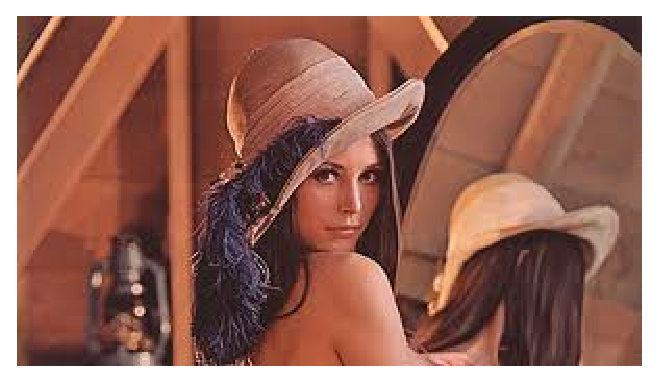
\includegraphics[scale=0.7]{Misc/TODO}
        \caption{}
        \label{Fig:3:FullSusceptibility}
    \end{center}
\end{figure}




\section{Discussion}

Similar differences between the measured data and calculations were observed for the sister 122 compound SrFe$_2$P$_2$\cite{Analytis2009} and is entirely consistent with results obtained on the entire \BaFePAs series\cite{Shishido2010}. Notably however, the non-nested 122 pnictide compound CaFe$_2$P$_2$ does not show any such differences to the DFT calculations, suggesting that perhaps the shifts in energy may arise from spin-fluctuations.

Orbital character is negligible for s and p orbitals for all bands which confirms ...

Energy shifts for band $2$ are proprtional to the \DzTwo and \DxzDyz characters, implies there may be a link between the \kz scattering and energy enhancements.


It is interesting to note that the DFT applied energy shifts apply to partially nested Fermi surfaces, whereas the large, unested portion of band 2 has zero shift. Other partially nested pnictide materials such as LaFePO\cite{Carrington2009} and SrFe$_{2}$P$_{2}$\cite{Analytis2009} have similar shifts whereas the non-nested, material CaFe$_{2}$P$_{2}$\cite{Coldea2009} matches the DFT calculations well without any rigid energy shift. This correlation between nesting and corrections to the DFT calculation lends weight to the notion that the shifts in the calculation energies are cause by spin fluctuations.





\section{Conclusions}

Similar differences between the measured data and calculations were observed for the sister 122 compound SrFe$_2$P$_2$\cite{Analytis2009} and is entirely consistent with results obtained on the entire \BaFePAs series\cite{Shishido2010}. Notably however, the non-nested 122 pnictide compound CaFe$_2$P$_2$ does not show any such differences to the DFT calculations, suggesting that perhaps the shifts in energy may arise from spin-fluctuations.

Orbital character is negligible for s and p orbitals for all bands which confirms ...

Energy shifts for band $2$ are proprtional to the \DzTwo and \DxzDyz characters, implies there may be a link between the \kz scattering and energy enhancements.


It is interesting to note that the DFT applied energy shifts apply to partially nested Fermi surfaces, whereas the large, unested portion of band 2 has zero shift. Other partially nested pnictide materials such as LaFePO\cite{Carrington2009} and SrFe$_{2}$P$_{2}$\cite{Analytis2009} have similar shifts whereas the non-nested, material CaFe$_{2}$P$_{2}$\cite{Coldea2009} matches the DFT calculations well without any rigid energy shift. This correlation between nesting and corrections to the DFT calculation lends weight to the notion that the shifts in the calculation energies are cause by spin fluctuations.





% \chapter{Hall measurements on \BSCO}


\section{Field sweeps}




\section{Conclusions}





% \chapter{Magnetoresistance measurements on \BSCO}


\section{Temperature sweeps}




\section{Field Sweeps}




\section{Conclusions}





% Bibliography
\clearpage

\thebibliography


% Appendix here

\end{document}
